Here, we show qualitative video comparisons of our reconstruction results to other methods to visually demonstrate the impact of our approach. Additional qualitative results for our novel view synthesis results are also included, and finally we conclude with some additional experimental details on our evaluation datasets of DTU \cite{aanaes2016large} and BlendedMVS \cite{yao2020blendedmvs} as well as additional implementation details.
\\
\noindent \textbf{Implementation Details.}
Following~\cite{liu2024fast}, for depth estimation, we sample $64$ and $8$ depth planes for the coarse and fine stages, respectively.
We set $\lambda_s=0.1$, $\lambda_p=0.05$, $\lambda_\alpha=0.05$, $\lambda_\beta=0.05$ and $\lambda_\gamma=0.05$, $\lambda^1=0.5$ and $\lambda^2=1$ for our loss weights.

\section{Additional qualitative comparison on 3D reconstruction}
Based on our $3$D reconstruction experiments, we have included some additional video visualizations of our surface reconstructions in the included supplementary material. There's $1$ on DTU \cite{aanaes2016large}, namely DTU\_Scan$122$.mp4 and $1$ on BlendedMVS \cite{yao2020blendedmvs}, namely BMVS\_Scan$2$.mp4. We also have a video result for the novel view synthesis task, namely NVS\_scan$1$.mp4

\section{Additional qualitative comparison on Novel View Synthesis}
In this section, we present additional qualitative comparisons with MVSGaussian \cite{liu2024fast} in Figure \ref{fig:nvs_grid_additional} to demonstrate the superior performance of our method on the DTU \cite{aanaes2016large} dataset. Our final adapted model exceeds the novel-view capabilities of its initial backbone to achieve SOTA performance and provides good novel-view extrapolation results compared to the generalizable reconstruction networks, which generally exhibit poor NVS performance (as pointed out in GeoTransfer \cite{jena2024geotransfer} supplementary). We notice that qualitatively, in the sparse $3$ input views setting, we are sharper than previous SOTA MVSGaussian \cite{liu2024fast}, with lesser artifacts. This demonstrates the robustness of our method on the task of novel-view synthesis, apart from also displaying \textbf{state-of-the-art} results on surface reconstruction. 

\begin{figure*}[t]
    \centering
    \setlength{\tabcolsep}{1pt}
    \begin{minipage}{\linewidth}
    \centering
    \begin{tabular}{@{}cccccc@{}}
        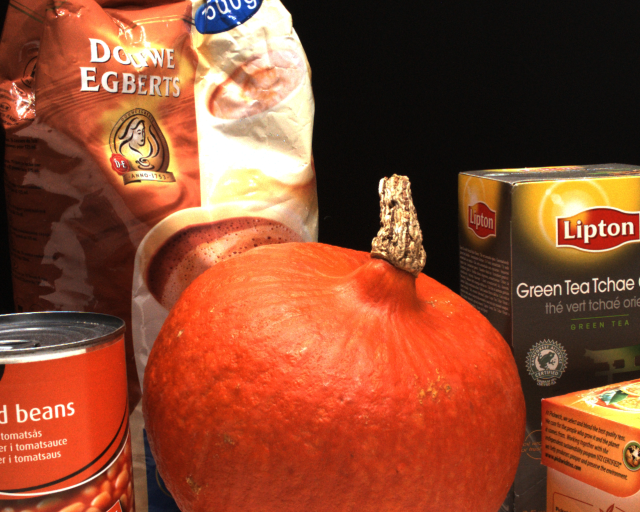
\includegraphics[width=0.162\linewidth]{figs/NVS/scan31_44_0_gt.png} & 
        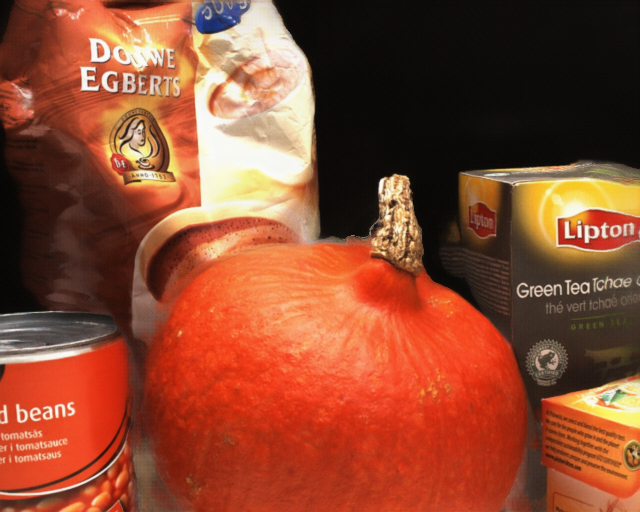
\includegraphics[width=0.162\linewidth]{figs/NVS/scan31_44_0_pred_mvsgs.png} & 
        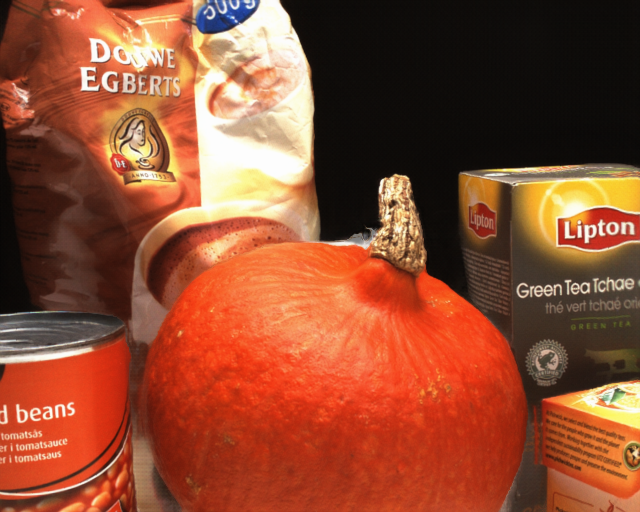
\includegraphics[width=0.162\linewidth]{figs/NVS/scan31_44_0_pred_ours.png} &
        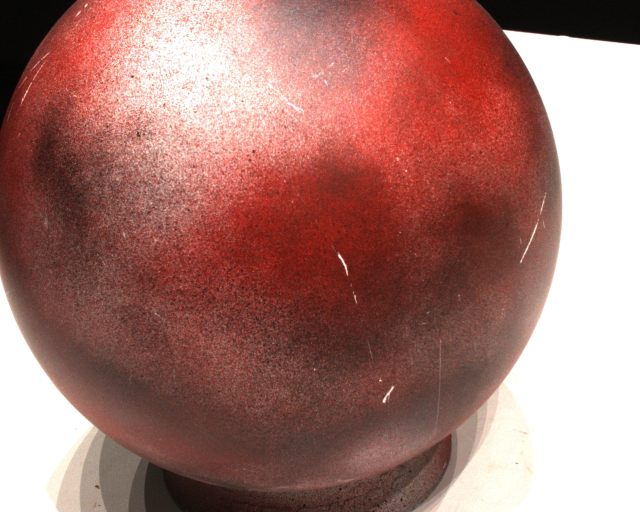
\includegraphics[width=0.162\linewidth]{figs/NVS/scan8_24_0_gt.png} & 
        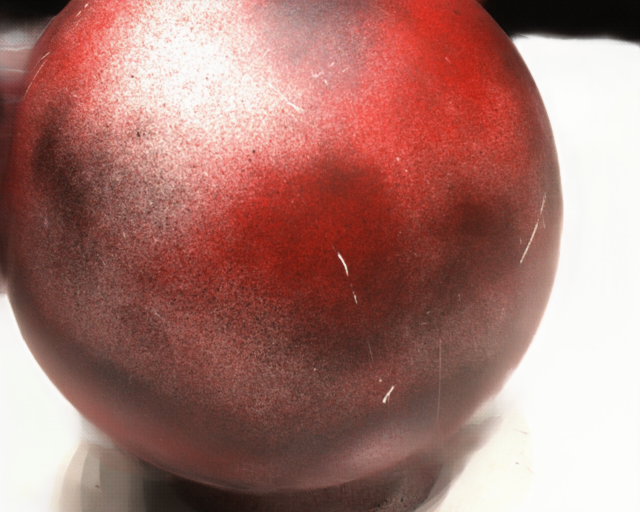
\includegraphics[width=0.162\linewidth]{figs/NVS/scan8_24_0_pred_mvsgs.png} & 
        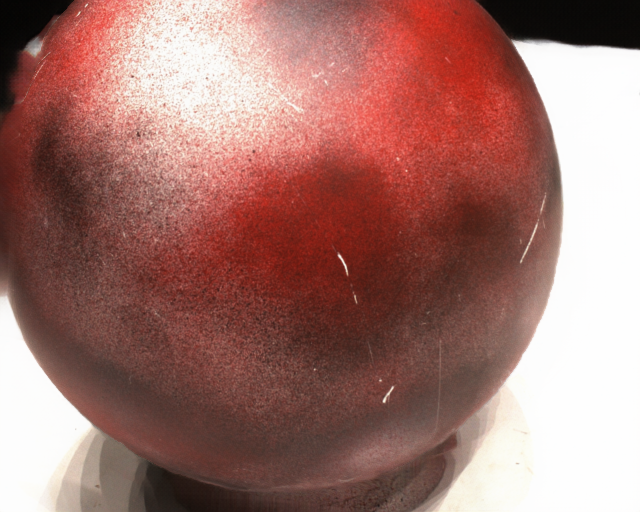
\includegraphics[width=0.162\linewidth]{figs/NVS/scan8_24_0_pred_ours.png} \\
        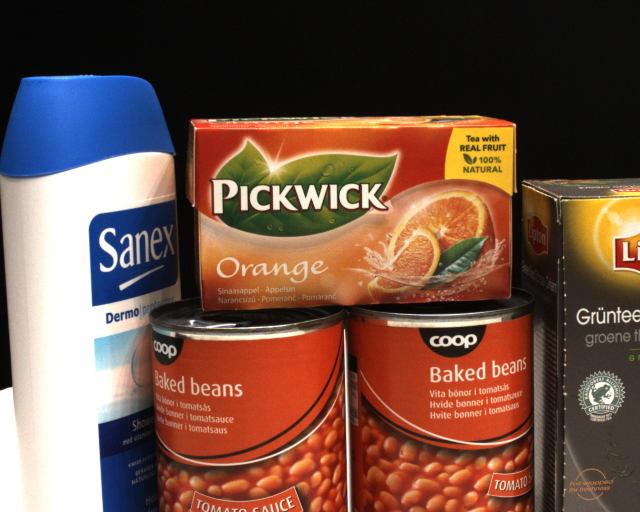
\includegraphics[width=0.162\linewidth]{figs/NVS/scan45_44_0_gt.png} & 
        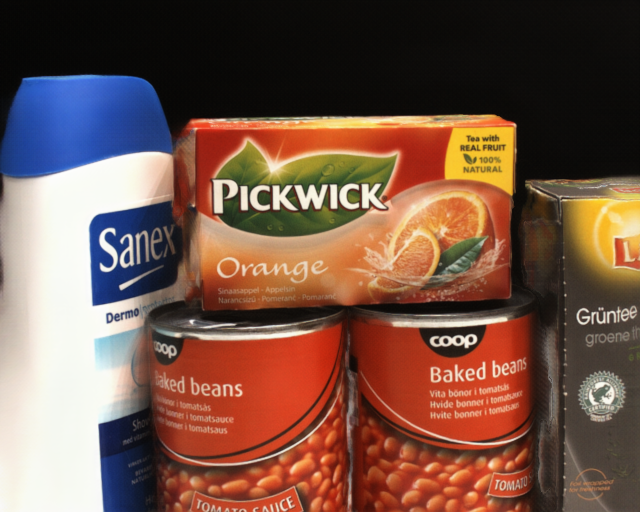
\includegraphics[width=0.162\linewidth]{figs/NVS/scan45_44_0_pred_mvsgs.png} & 
        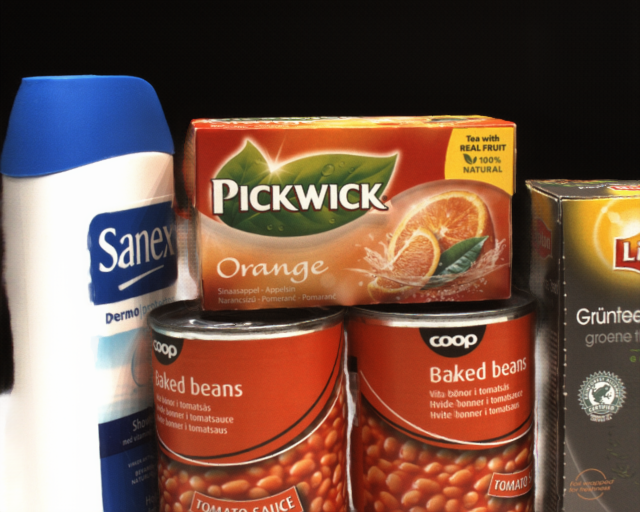
\includegraphics[width=0.162\linewidth]{figs/NVS/scan45_44_0_pred_ours.png} & 
        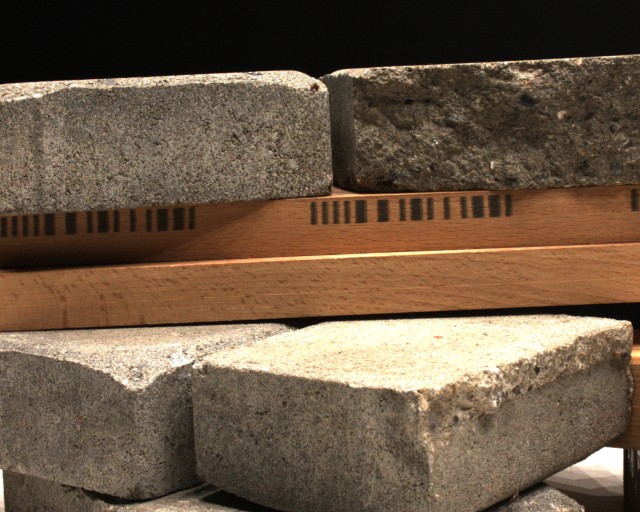
\includegraphics[width=0.162\linewidth]{figs/NVS/scan38_44_0_gt.png} & 
        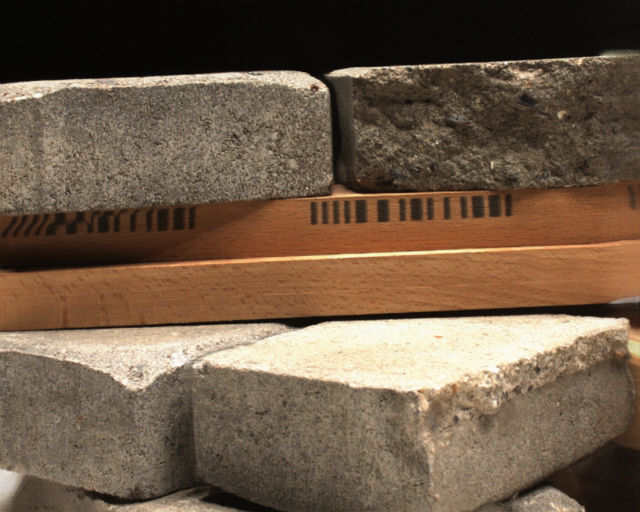
\includegraphics[width=0.162\linewidth]{figs/NVS/scan38_44_0_pred_mvsgs.png} & 
        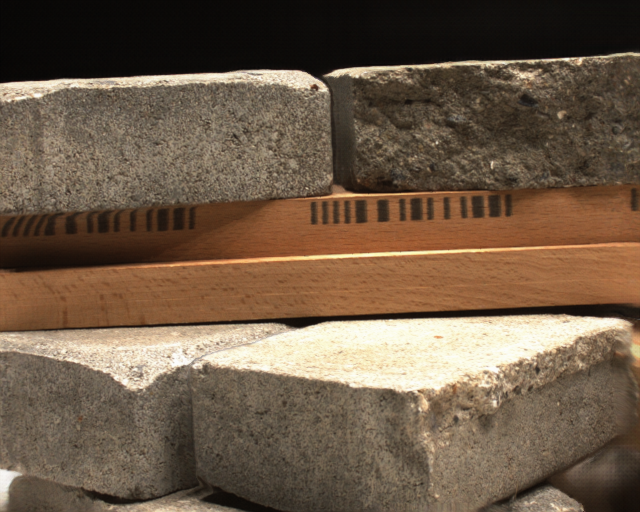
\includegraphics[width=0.162\linewidth]{figs/NVS/scan38_44_0_pred_ours.png} \\
        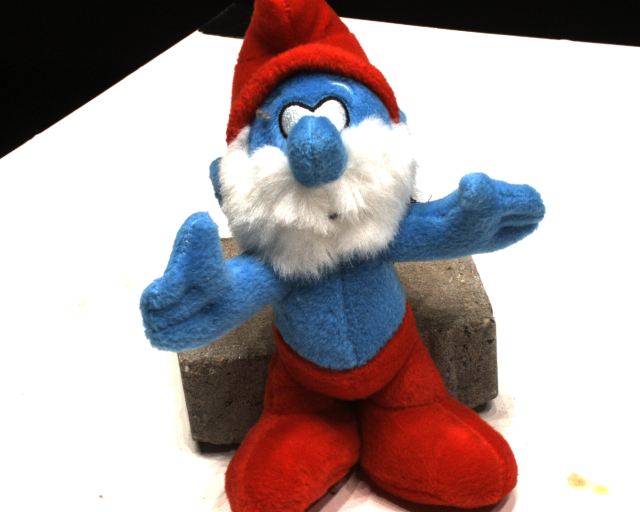
\includegraphics[width=0.162\linewidth]{figs/NVS/scan82_24_0_gt.png} & 
        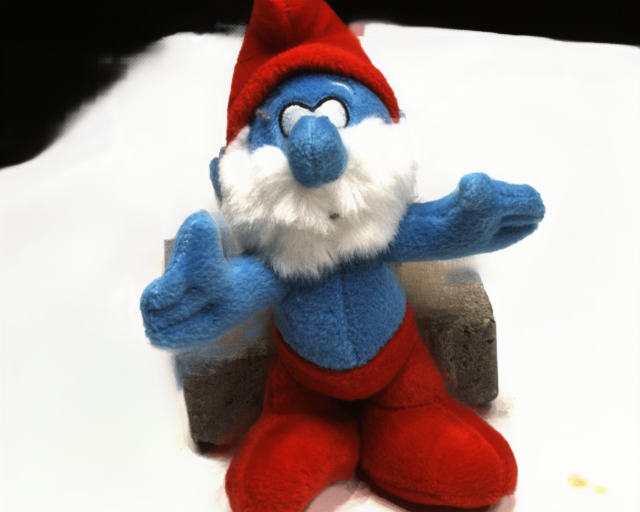
\includegraphics[width=0.162\linewidth]{figs/NVS/scan82_24_0_pred_mvsgs.png} & 
        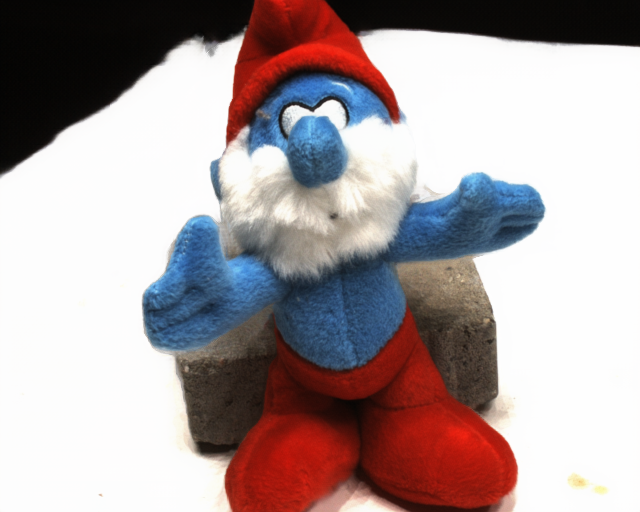
\includegraphics[width=0.162\linewidth]{figs/NVS/scan82_24_0_pred_ours.png} &
        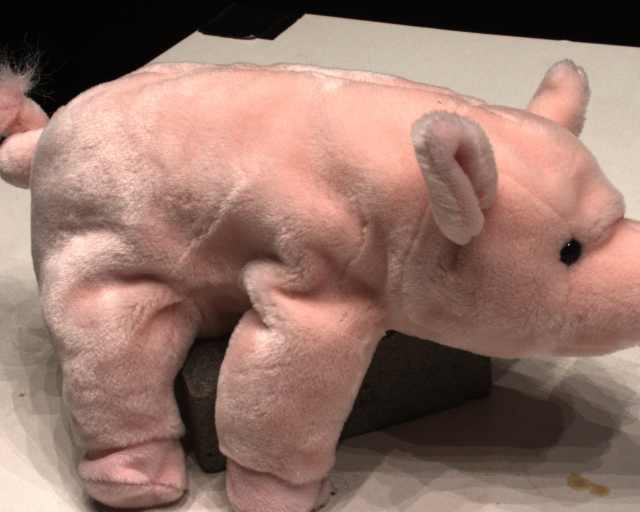
\includegraphics[width=0.162\linewidth]{figs/NVS/scan103_24_0_gt.png} & 
        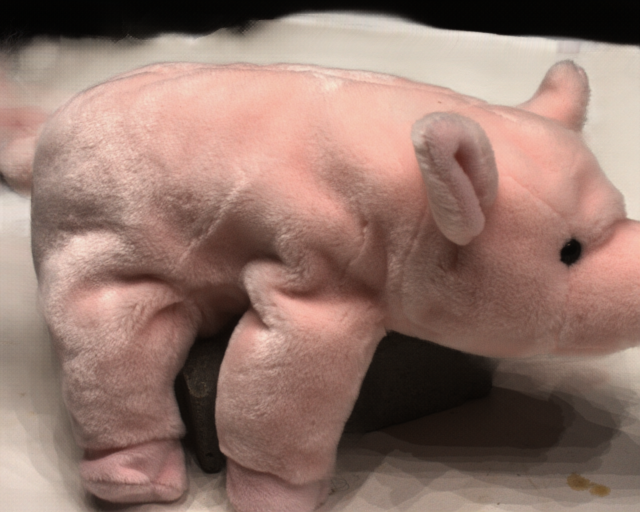
\includegraphics[width=0.162\linewidth]{figs/NVS/scan103_24_0_pred_mvsgs.png} & 
        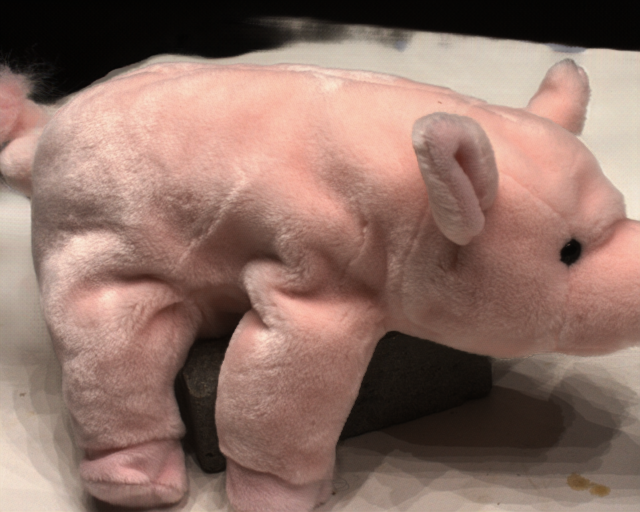
\includegraphics[width=0.162\linewidth]{figs/NVS/scan103_24_0_pred_ours.png} \\
        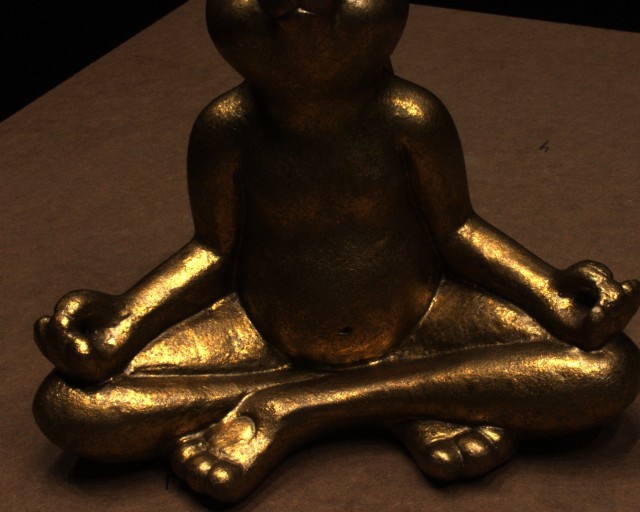
\includegraphics[width=0.162\linewidth]{figs/NVS/scan110_24_0_gt.png} & 
        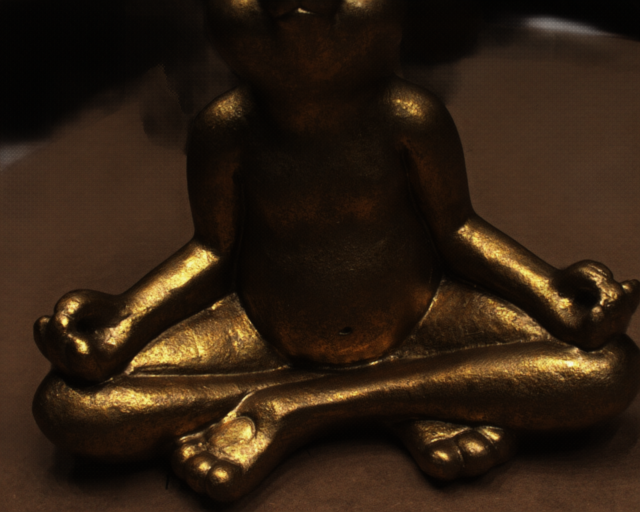
\includegraphics[width=0.162\linewidth]{figs/NVS/scan110_24_0_pred_mvsgs.png} & 
        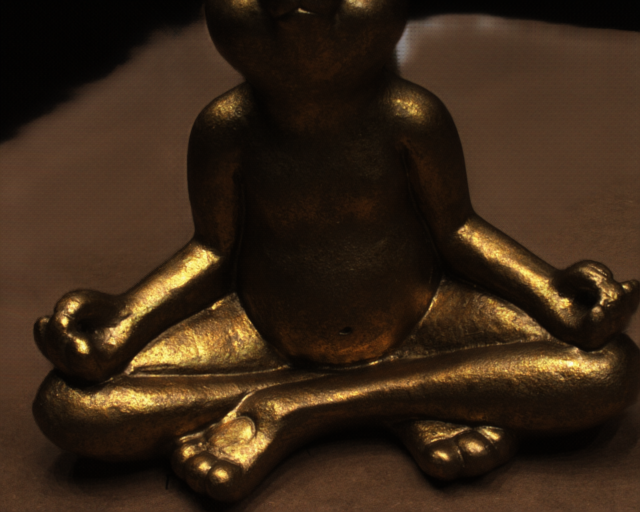
\includegraphics[width=0.162\linewidth]{figs/NVS/scan110_24_0_pred_ours.png} & 
        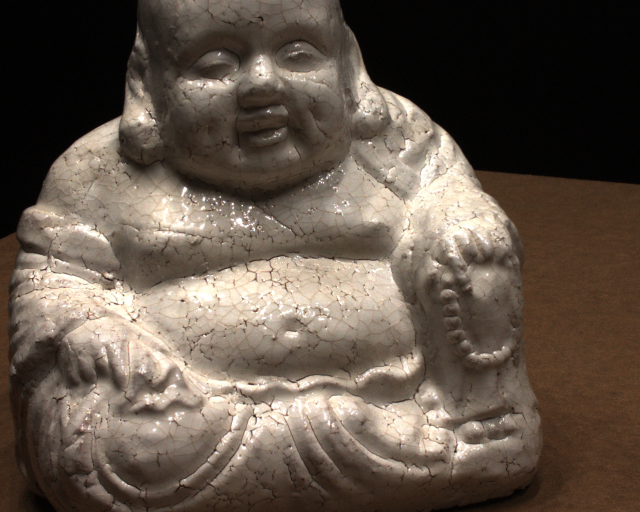
\includegraphics[width=0.162\linewidth]{figs/NVS/scan114_32_0_gt.png} & 
        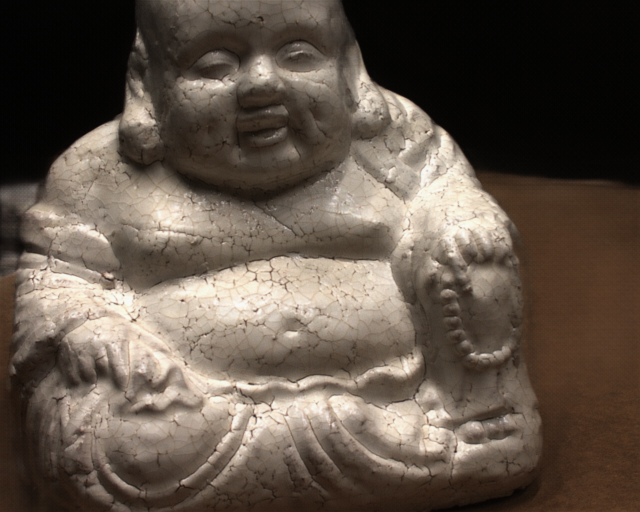
\includegraphics[width=0.162\linewidth]{figs/NVS/scan114_32_0_pred_mvsgs.png} & 
        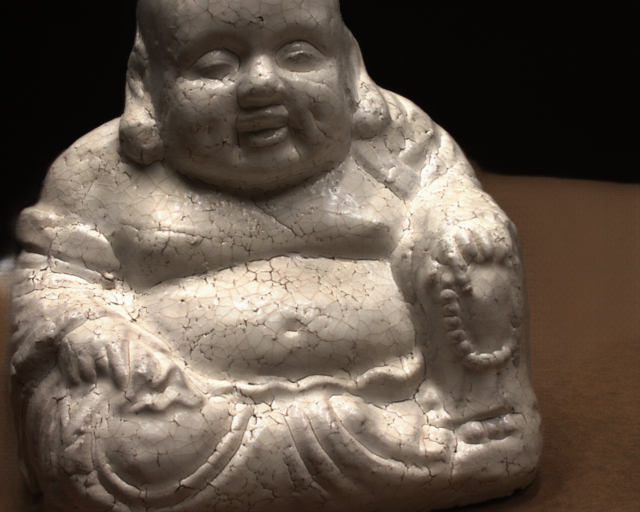
\includegraphics[width=0.162\linewidth]{figs/NVS/scan114_32_0_pred_ours.png} \\
        GT & MVSGaussian \cite{liu2024fast} & Ours & GT & MVSGaussian \cite{liu2024fast} & Ours \\
    \end{tabular}
    \end{minipage}
    \caption{Additional Novel-View synthesis qualitative evalutation on DTU \cite{aanaes2016large} using $3$ source images. We outperform SOTA MVSGaussian \cite{liu2024fast} and exhibit sharper view synthesis results, particularly on object boundaries.}
    \label{fig:nvs_grid_additional}
\end{figure*}

\section{Additional Experimental Details}
\label{sec:exp_details}
In this work, we evaluated two sets of data: DTU \cite{aanaes2016large} and BlendedMVS \cite{yao2020blendedmvs}. For DTU \cite{aanaes2016large}, we follow distinct protocols based on the task's nature, distinguishing between novel view synthesis and surface reconstruction.

\paragraph{\textbf{Metrics}} For the novel view synthesis task involve evaluating PSNR scores, assuming a maximum pixel value of 1 and using the formula $-10 \log_{10}$(MSE). Additionally, we employ the scikit-image's API to calculate the Structural Similarity Index (SSIM) score and the pip package lpips, utilizing a learned VGG model for computing the Learned Perceptual Image Patch Similarity (LPIPS) score. In the context of the surface reconstruction task, we gauge Chamfer Distances by comparing predicted meshes with the ground truth point clouds of DTU scans. The evaluation process follows the methodology employed by SparseNeuS, VolRecon, ReTR, GeoTransfer \cite{long2022sparseneus, ren2023volrecon, liang2024retr, jena2024geotransfer}, employing an evaluation script that refines generated meshes using provided object masks. Subsequently, the script evaluates the chamfer distance between sampled points on the generated meshes and the ground truth point cloud, producing distances in both directions before providing an overall average, typically reported in evaluations. Additionally, two sets of 3 different views are used for each scan, and we average the results between the two resulting meshes from each set of images and report it in the comparison as done in previous methods \cite{long2022sparseneus, ren2023volrecon, liang2024retr, jena2024geotransfer}.

\paragraph{\textbf{DTU Dataset}} The DTU dataset \cite{aanaes2016large} is an extensive multi-view dataset comprising $124$ scans featuring various objects. Each scene is composed of $49$–$64$ views with a resolution of $1600 \times 1200$. We adhere to the procedure outlined in \cite{long2022sparseneus, ren2023volrecon, liang2024retr}, training on the same scenes as employed in these methods and then test on the $15$ designated test scenes the reconstruction task. The test scan IDs surface reconstruction are : $24$, $37$, $40$, $55$, $63$, $192$, $65$, $69$, $83$, $97$, $105$, $106$, $110$, $114$, $118$ and $122$. For surface reconstruction, for each scan, there are two sets of 3 views with the following IDs used as the input views: set-$0$: $23$, $24$ and $33$, then set-$1$: $42$, $43$ and $44$ all scans. We use the training views in the resolution, \ie $640 \times 512$. For the task of novel view synthesis, we use the same split of training and testing views as MVSGaussian \cite{liu2024fast} as well as adopt the same input view set as them for fairness of comparison. 

\paragraph{\textbf{BlendedMVS Dataset}} BlendedMVS \cite{yao2020blendedmvs} is a large-scale dataset for generalized multi-view stereo that consists of a variety of $113$ scenes including architectures, sculptures and small objects with complex backgrounds. For surface-reconstruction, we use $4$ challenging scenes, where each scene has $31$–$143$ images captured at $768 \times 576$.